\section{Auswertung}
\label{sec:Auswertung}

\subsection{Messung bis 1 bar}

Zur Berechnung der Verdampfungswärme $L$ wird die in (\ref{eq:damppfdruck}) hergeleitete Gleichung 
\begin{equation}
    \ln \left(\frac{p}{p_{0}}\right) = -\frac{L}{R} \cdot \frac{1}{T}
\end{equation}
verwendet. Der zu Beginn gemesse Umgebungsdruck beträgt dabei
\begin{equation}
    p_{0} = \qty{1013e2}{kPa} \, .
\end{equation}

Aus den gemessenen Wertepaaren $(p,T)$ und einer linearen Ausgleichsrechnung
wird mittels SCIPY \cite{scipy} die Ausgleichsgerade der Form
\begin{equation}
    y = ax + b 
\end{equation}
in Abbildung \ref{fig:plot1} dargestellt.
Es sei angemerkt, dass aufgrund von Problemen bei der Messung einige Daten nicht aufgezeichnet wurden,
was die Lücke bei der Messreihe erklärt.
\begin{figure}[H]
    \centering
    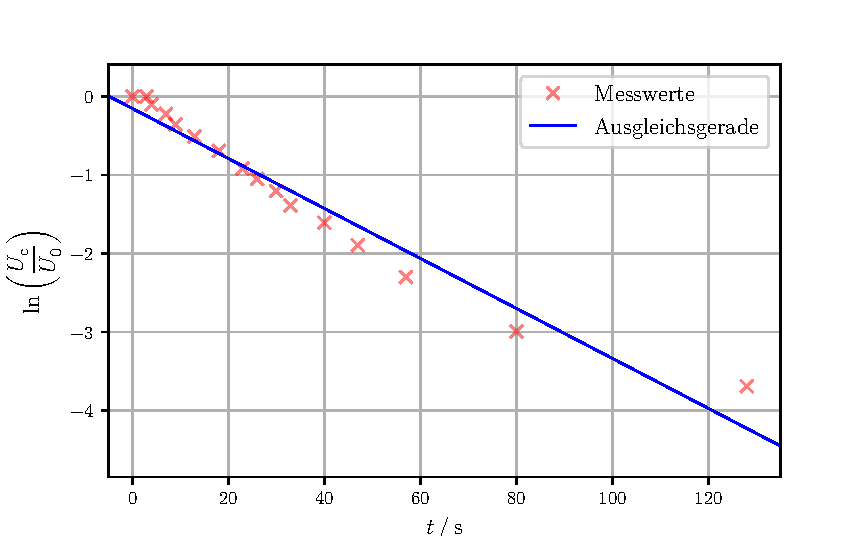
\includegraphics[width=\textwidth]{plot1.pdf}
    \caption{Ausgleichsgerade im Druckbereich $p \leq \qty{1}{bar}$.}
    \label{fig:plot1}
\end{figure}

Für die Parameter ergeben sich somit
\begin{align*}
    a &= \num{-3.225(060)e3} \quad \text{und} \\
    b &= \num{15.38(17)} \, .
\end{align*}

Wird die Beziehung der Steigung $a$ aus (\ref{eq:damppfdruck}) verwendet, lässt sich $L$ damit durch
\begin{equation}
    a = -\frac{L}{R} \quad \Rightarrow \quad L=-a \cdot R
\end{equation}
ausdrücken. 
Somit ergibt sich die Verdampfungswärme zu
\begin{equation}
    L = \qty{26.8(5)}{\kilo\joule\per\mol} \, .
\end{equation}

Die äußere Verdampfungswärme $L_\text{a}$ ist die benötigte Energie, 
um das Volumen eines Mols der Flüssigkeit auf das Volumen eines Mols des Gases zu vergrößern.
Wird die dabei verrichtete Volumenarbeit $W = pV$  gleich der idealen Gasgleichung (\ref{eq:idgasgleichung})
gesetzt, ergibt sich bei $T = \qty{373}{K}$ für die äußere Verdampfungswärme
\begin{equation}
    L_{\text{a}} = W = pV = RT = \qty{3.101}{\kilo\joule\per\mol} \text{ .}
\end{equation}

Die benötigte innere Energie $L_\text{i}$ um die molekularen Bindungskräfte bei der Verdampfung zu überwinden ist damit
\begin{equation}
    L_{\mathrm{i}} = L-L_{\mathrm{a}} = \qty{23.7(5)}{\kilo\joule\per\mol} \, .
\end{equation}

Eine Division durch die Avogadro-Konstante $N_\text{A} = \qty{6.022e23}{\per\mol}$
ergibt die innere Energie pro Molekül. Somit lautet das Ergebnis in Elektronenvolt
\begin{equation}
    L_{\text{i}} = \qty{0.246(5)}{\eV} \, .
\end{equation}


\subsection{Messung von 1 bis 15 bar}

Mithilfe der Messdaten im Druckbereich $p \in [1, 15] \, \mathrm{bar}$ soll nun die Temperaturabhängigkeit
der Verdampfungswärme $L$ untersucht werden. Dafür wird (\ref{eq:clausius}) nach $L$ umgestellt. Es gilt
\begin{equation}
    L = T \left(V_{\text{D}} - V_{\text{F}}\right) \frac {\dif{p}} {\dif{T}} \, . \label{eq:verdampfungswärme}
\end{equation}

Obwohl $V_\text{F}$ weiterhin vernachlässigbar ist, kann $V_\text{D}$ nicht mehr durch (\ref{eq:idgasgleichung})
ausgedrückt werden.
Eine bessere Näherung stellt die Gleichung
\begin{equation}
    \left(p + \frac {A} {V_{\text{D}}^{2}}\right) V_{\text{D}} = RT 
    \quad \text { mit } \quad
    A = \qty[per-mode=fraction]{0.9}{\joule\m\cubed\per\mol\squared} 
\end{equation}
\begin{equation}
    \Rightarrow \quad V_{\text{D}} = \frac{RT}{2p} \pm \sqrt{ \frac {R^{2} T^{2}} {4 p^{2}} - \frac{A}{p} } 
\end{equation}
dar. Somit ergibt sich für (\ref{eq:verdampfungswärme}) 
\begin{equation}
    L = T\left[\frac{R T}{2 p} \pm \sqrt{\frac{R^{2} T^{2}}{4 p^{2}}-\frac{A}{p}}\right] \frac{\dif{p}}{\dif{T}} 
    = \frac{T}{p} \left[\frac{R T}{2} \pm \sqrt{\left(\frac{R T}{2}\right)^{2}-A p}\right] \frac{\dif{p}}{\dif{T}} \, .
    \label{eq:L}
\end{equation}

Um den auftretenden Differentialquotienten $\frac{\dif{p}}{\dif{T}}$ zu bestimmen,
wird aus den gemessenen Wertepaaren $(p,T)$ ein Ausgleichsploynom 3. Grades der Form
\begin{align*}
    p(T) &= a \cdot T^{3} + b \cdot T^{2} + c \cdot T+d \quad \text{bzw.} \\
    \frac{\dif{p}}{\dif{T}} &= 3a \cdot T^{2} + 2b \cdot T + c \quad 
\end{align*}
in Abbildung \ref{fig:plot2} dargestellt.
\begin{figure}[H]
    \centering
    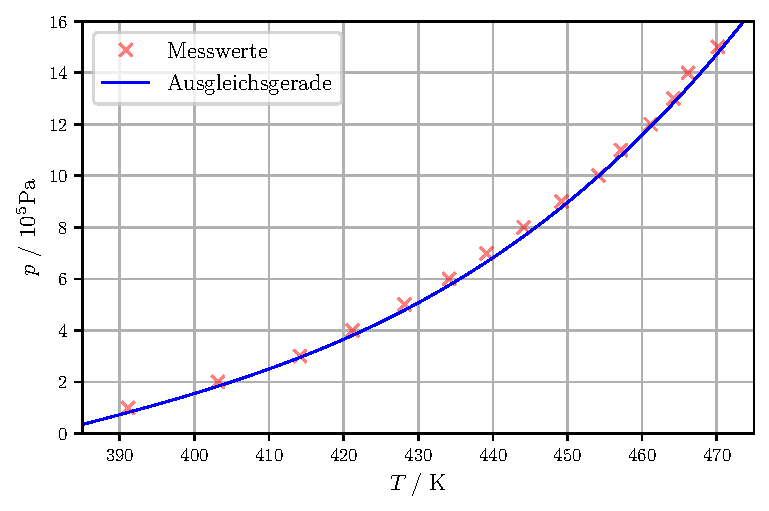
\includegraphics[width=\textwidth]{plot2.pdf}
    \caption{Ausgleichspolynom im Druckbereich $p \in [1, 15] \, \mathrm{bar}$.}
    \label{fig:plot2}
\end{figure}

Damit ergibt sich für die Parameter
\begin{align*}
    a &= \qty{1.108(341)}{\pascal\per\cubic\kelvin} \, , \\
    b &= \qty{-1.263(442)e3}{\pascal\per\kelvin\squared} \, , \\ % *10**3
    c &= \qty{4.877(1.903)e5}{\pascal\per\kelvin} \, \, \text{und} \\ % *10**5
    d &= \qty{-6.367(2.727)e7}{\pascal} \, . % *10**7
\end{align*}

Werden nun $p(T)$ und $\frac{\dif{p}}{\dif{T}}$ in \ref{eq:L} eingesetzt, 
ergibt sich die Gleichung 
\begin{align}
    L(T) &= \frac{T \left(3 a T^{2}+2 b T+c\right)}{a T^{3}+b T^{2}+c T+d} \left[\frac{R T}{2} \pm \sqrt{\left(\frac{R T}{2}\right)^{2}-A \left(a T^{3}+b T^{2}+c T+d\right)}\right]  \\
    &= \frac{3 a T^{3}+2 b T^{2}+c T}{a T^{3}+b T^{2}+c T+d} \left[\frac{R T}{2} \pm \sqrt{\left(\frac{R T}{2}\right)^{2}-A\left(a T^{3}+b T^{2}+c T+d\right)}\right] \text{ .}
\end{align}

Die daraus resultierenden temperaturabhängigen Verdampfungswärmen sind in den Abbildungen
\ref{fig:plot3} und \ref{fig:plot4} aufgetragen.

\begin{figure}[H]
    \centering
    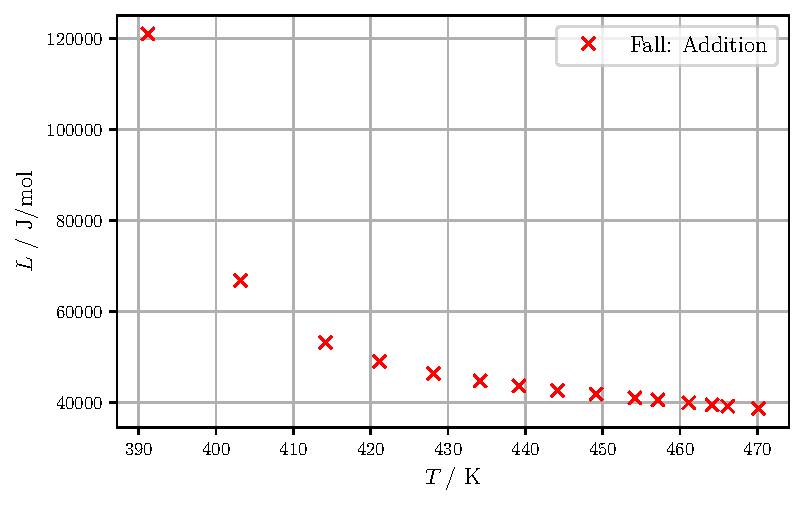
\includegraphics[width=0.9\textwidth]{plot3.pdf}
    \caption{Temperaturabhängigkeit der Verdampfungswärme im Falle der Addition.}
    \label{fig:plot3}
\end{figure}

\begin{figure}[H]
    \centering
    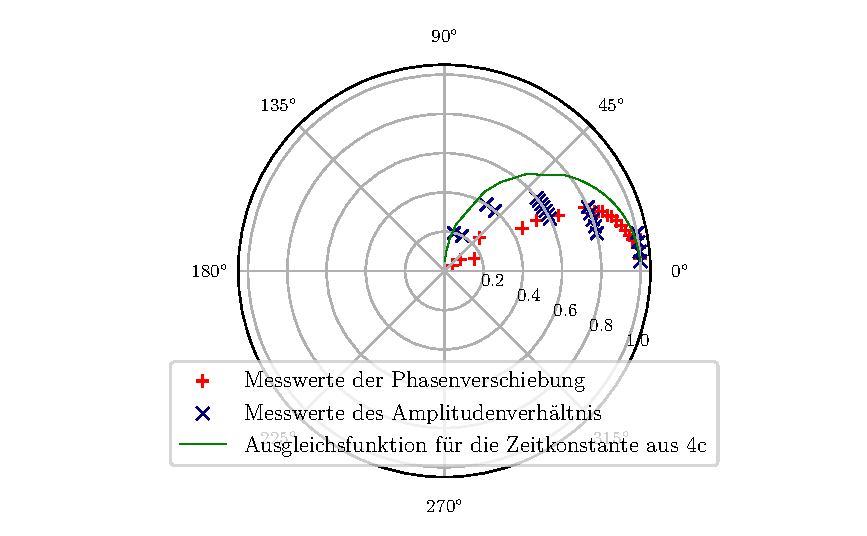
\includegraphics[width=0.9\textwidth]{plot4.pdf}
    \caption{Temperaturabhängigkeit der Verdampfungswärme im Falle der Subtraktion.}
    \label{fig:plot4}
\end{figure}